\subsection{\leo{Cycle Complexity Breakdown}}

Given the previous results, we embarked to investigate how to improve the
efficiency of the simple V-cycle with 1 relaxation step. The first step is to
breakdown the time spent in the different parts of a cycle. Note that all the
matrices for each level are computed in a setup phase and it is not necessary
to analyze that setup time. We only focus on measuring the following two
computations: (i) the time spent doing a relaxation at each level and (ii) the
time spent computing the next linear system. The latter (i.e., computing the
next linear system) can be divided in two options: \emph{going down} by
restricting the solution to a coarser grid, which corresponds to a sparse
matrix-vector computation; and \emph{going up} by interpolating the error term
which also corresponds to another sparse matrix-vector computation.

\begin{table}[htb]
 \resizebox{\linewidth}{!}{
 \begin{tabular}{|c|c|c|c|c|c|c|}
  \hline
  Level & \makecell{Matrix \\ size} & \makecell{Non-zero \\ elements} & \makecell{Relax \\ (down)} & \makecell{Relax \\ (up)} & \makecell{MatVec \\ (down)} & \makecell{MatVec \\ (up)} \\
  \hline
  1 & 512,000 & 4,042,520 & 20 ms & 20 ms & 15 ms & -\\
  \hline
  2 & 256,000 & 6,475,239 & 20 ms & 25 ms & 12 ms & 4 ms\\
  \hline
  3 & 58,893 & 2,000,513 & 8 ms & 8 ms & 3 ms & 2 ms\\
  \hline
  4 & 14,285 & 788,509 & 2 ms & 2 ms & 1 ms & 0.7 ms\\
  \hline
  5 & 4,238 & 386,333 & 1 ms & 1 ms & 0.5 ms & 0.2 ms\\
  \hline
  6 & 609 & 53,493 & $< 0.1$ ms & $< 0.1$ ms & $< 0.1$ ms & $< 0.1$ ms\\
  \hline
  7 & 69 & 2,873 & $< 0.1$ ms & $< 0.1$ ms & $< 0.1$ ms & $< 0.1$ ms\\
  \hline
  8 & 2 & 4 & $< 0.1$ ms & - & - & $< 0.1$ ms\\
  \hline
 \end{tabular}
 }
 \caption{Time breakdown of a V-cycle with $\alpha=1$.}
 \label{table.measures}
\end{table}

To study the internal time breakdown of a V-cycle we chose as problem an
unstructured domain with some anisotropy (denoted as Unstructured-Anisotropy)
of size 512,000 with a 8-level grid. The results of this evaluations are
depicted in Table~\ref{table.measures}, along with information on the matrix
used at the corresponding level, such as matrix size and the number of non-zero
elements.  Our first observation is that there is a direct correlation between
the time spent on relaxations at each given level and the number of non-zero
entries in the input matrix. Most importantly, in these results we observe that
relaxations represent $\approx66\%$ of the total cost of a V-cycle, while the
matrix-vector multiplications are only $\approx30\%$. In addition, we notice
that the two first levels are the most expensive ones.  It is important to
highlight that in the experiments depicted in Figure~\ref{fig.first_tests},
although different number of relaxations were evaluated, all levels executed
the \emph{same} number of relaxations.

\subsection{\leo{Level-Dependent Relaxation Tuning}}

Based on this information, we propose to reduce the execution time of a V-cycle
by tuning the number of relaxations differently for each level. More precisely
we propose the following two ideas: (i) to add more relaxations in the last
levels because their cost is negligible and they could potentially reduce the
time to convergence or (ii) to remove some relaxations in the first levels to
reduce the computational cost, and see how that affects convergence. We
translate these ideas into the four following strategies (based on a 8-level
grid):

\begin{itemize}
    \item \emph{Fast } : no relaxations at level 2.
    \item \emph{Fast2} : 10 relaxations at level 6.
    \item \emph{Fast3} :  2 relaxations at levels 6 and 4.
    \item \emph{Fast4} : no relaxations at level 3.
\end{itemize}

\begin{figure*}
    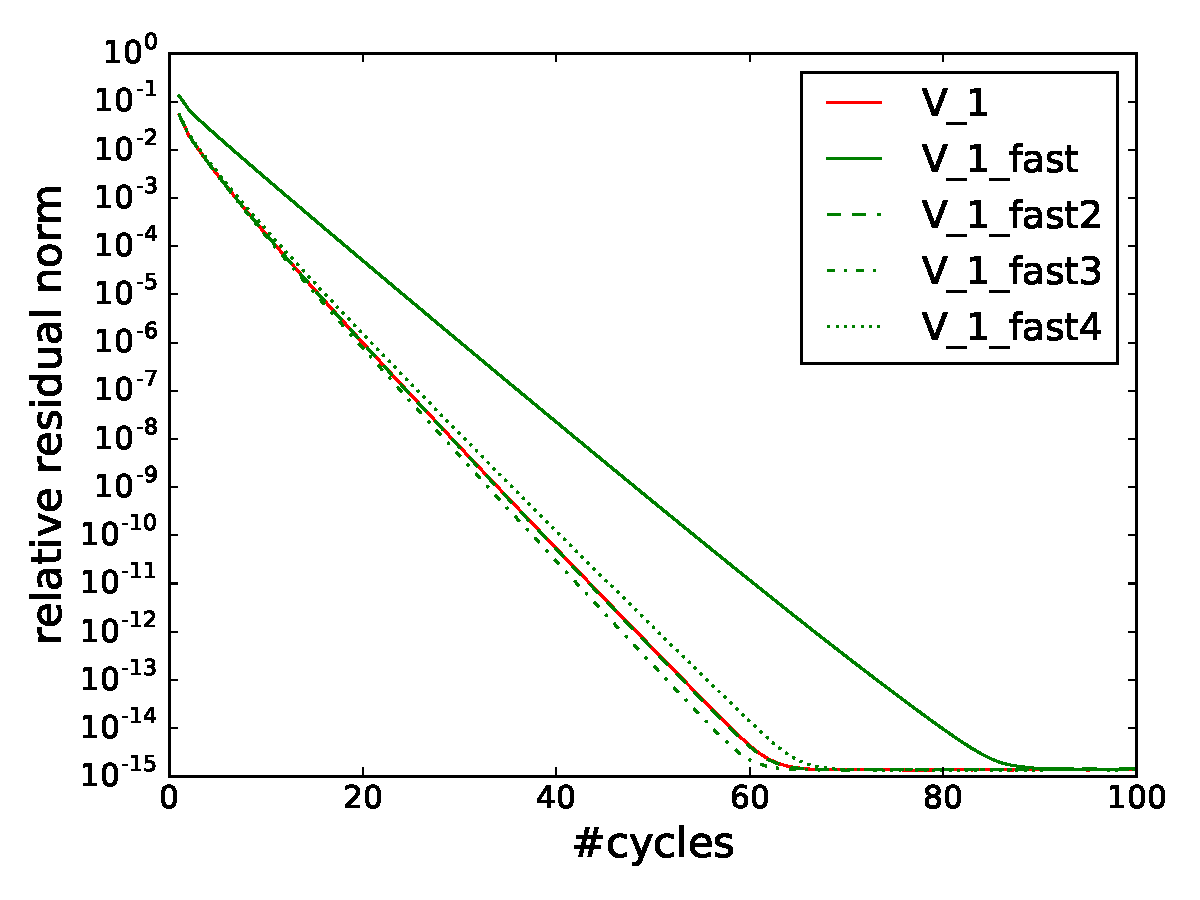
\includegraphics[width=0.33\linewidth]{figs/convergence_fast_norm.pdf}
    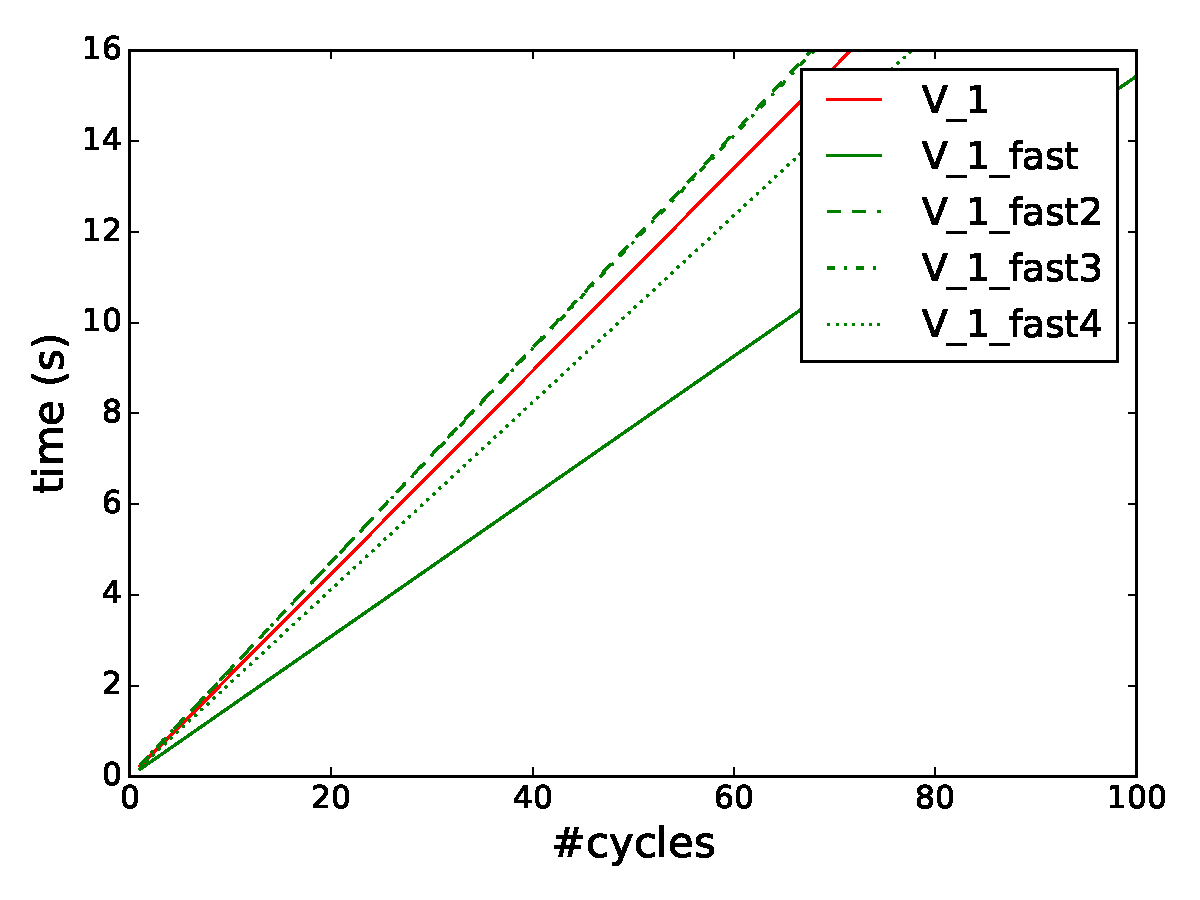
\includegraphics[width=0.33\linewidth]{figs/convergence_fast_time.pdf}
    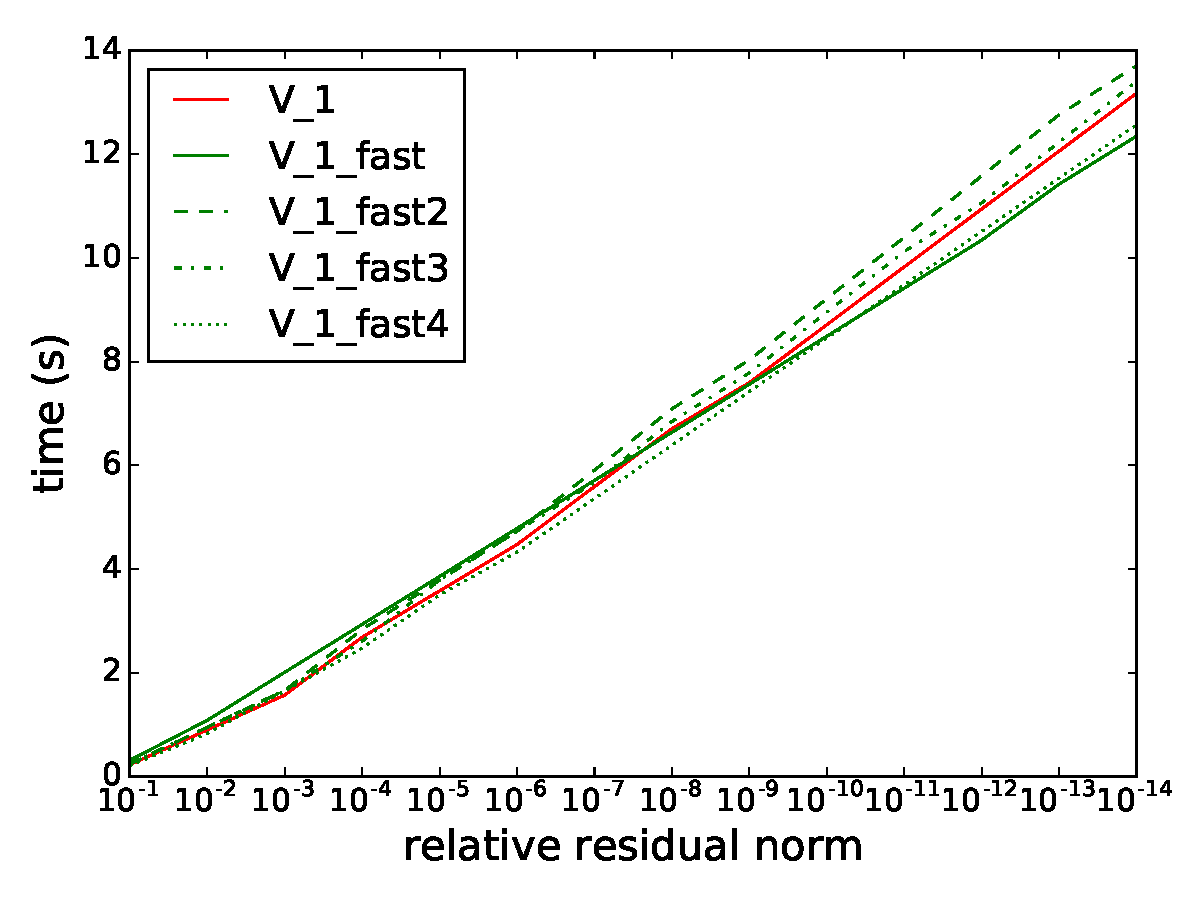
\includegraphics[width=0.33\linewidth]{figs/time_convergence_fast.pdf}
    \caption{Evaluation of 4 level-dependent relaxation tuning strategies.
    Residual norm per cycle (left), time spent in each cycle (middle) and
    convergence time in function of the error tolerance (right).}
    \label{fig.newstrat}
\end{figure*}

The strategy \emph{Fast} aims at reducing the cost of the cycle by removing the
penultimate relaxation which is very expensive, and expecting that the accuracy
lost at this point can be compensated by the relaxation at level 1.  The
strategy \emph{Fast2} executes a lot of relaxations at level 6, because it
should not increase by much the execution time of the V-cycle.  The reason to
choose level 6 instead of level 7 or 8 is that the relaxation at level 8 is
actually a direct solve. Thus, the result term is almost exact at level 7,
because the only source of error comes from the interpolation of $e^8$ (which
is exact) into $e^7$. This is why, we might expect better results by adding
relaxations at level 6. The strategy \emph{Fast3}, pushes the previous idea one
step further. If we assume that doing more than one relaxation gets a more
accurate error estimation at level $l$, then at level $l-1$ we do not need to
correct a lot by doing more relaxations. However at level $l-2$ we have been
through 2 interpolations since the last good estimation of the error vector,
therefore we increase the number of relaxations again. Since the first levels
are very expensive, we stop this recursion at level 3.  Finally, we propose one
last strategy \emph{Fast4} which is a softer version of \emph{Fast} where the
relaxation at level 3 is removed, producing a less accurate result at that
point, but expecting it can be compensated by the two relaxations at level 1
and 2.

%\begin{figure*}
%    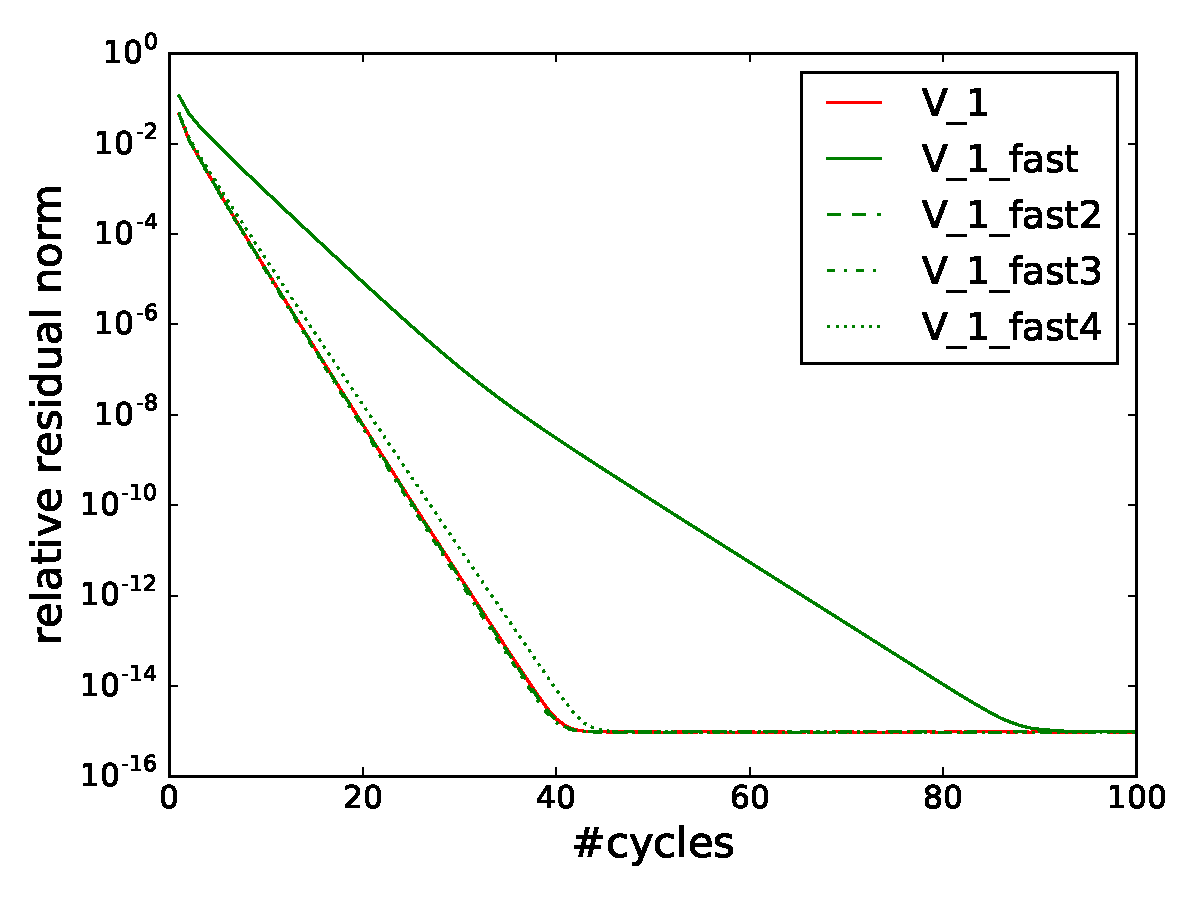
\includegraphics[width=0.33\linewidth]{figs/convergence_fast_small_norm.pdf}
%    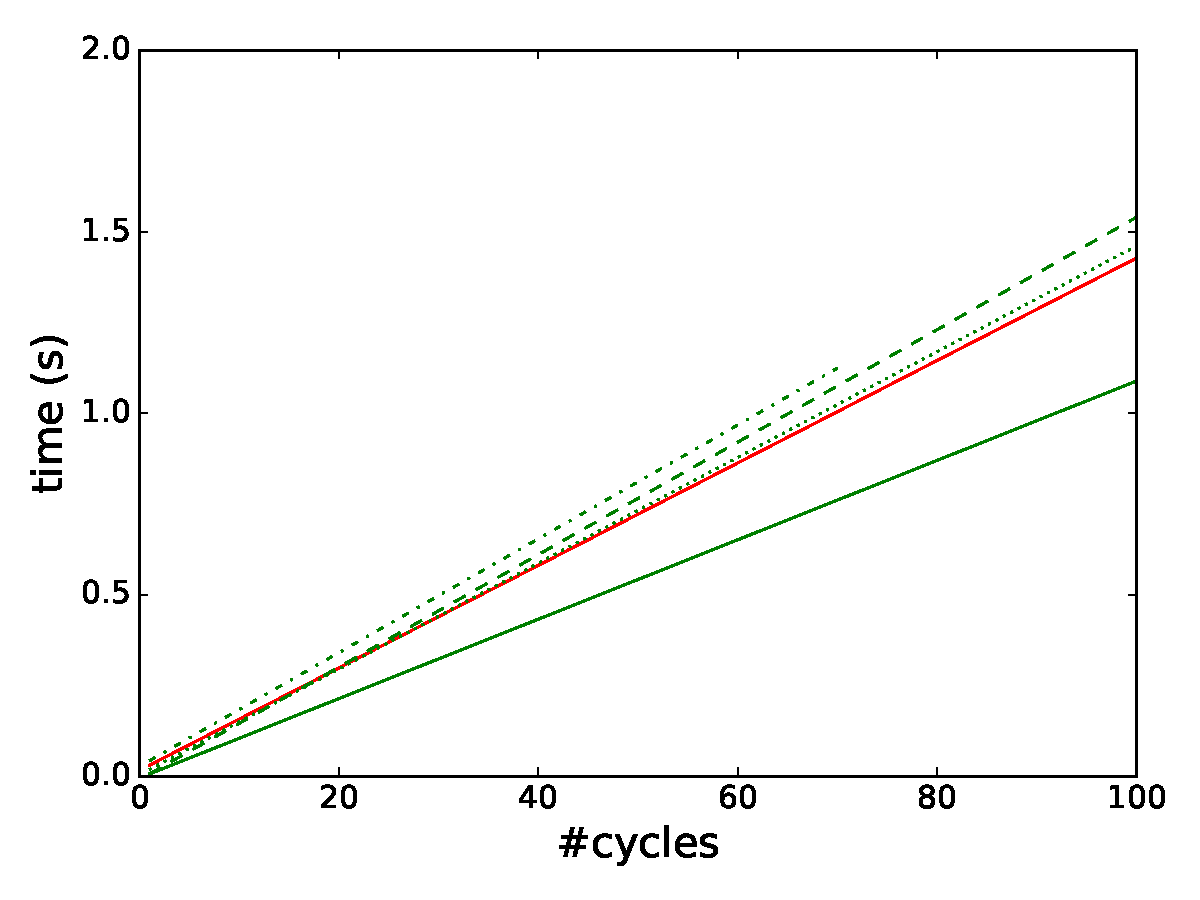
\includegraphics[width=0.33\linewidth]{figs/convergence_fast_small_time.pdf}
%    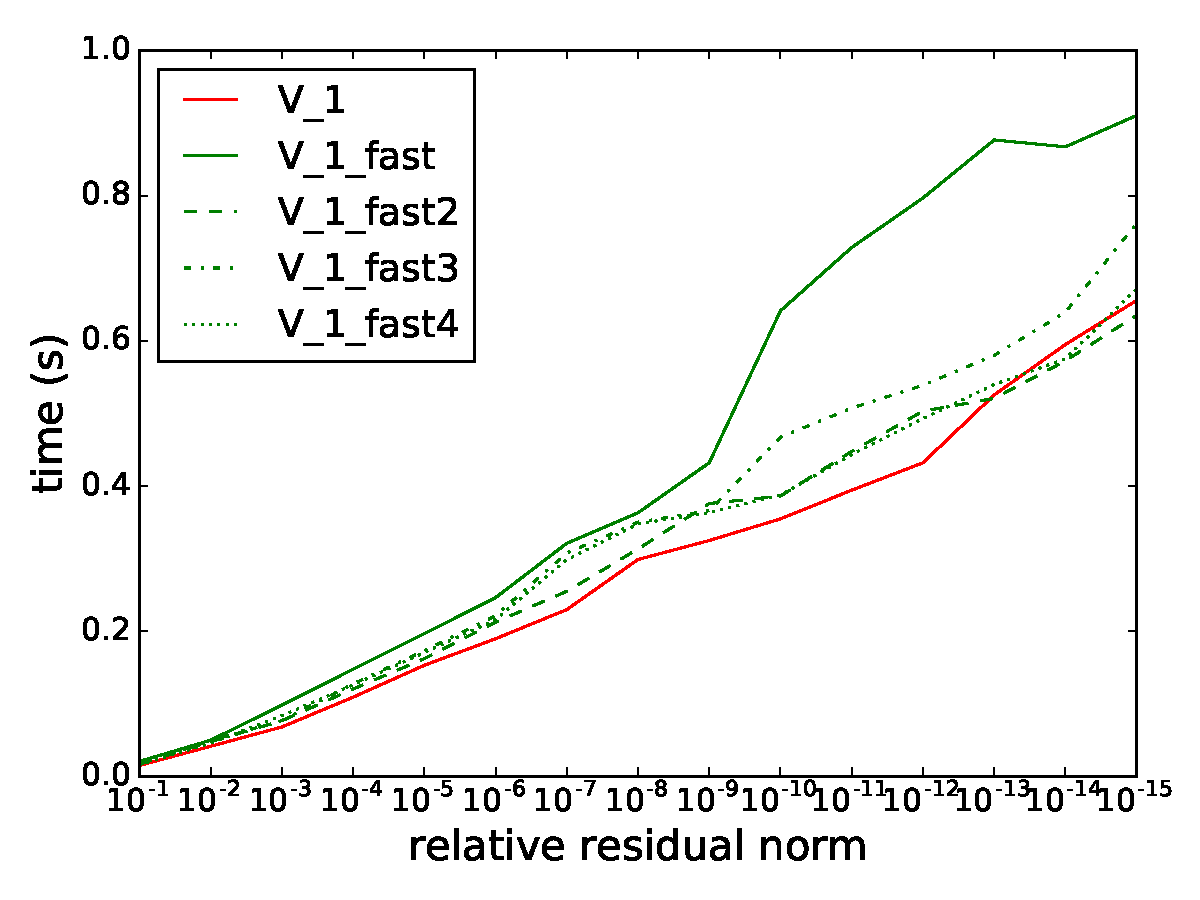
\includegraphics[width=0.33\linewidth]{figs/time_convergence_fast_small.pdf}
%    \caption{Final residual norm of the 4 new strategies per iteration (left),
%    interpolated execution time per iteration (middle) and convergence time as
%    a function of the tolerance (right) on a small matrix.}
%    \label{fig.newstrat_small}
%\end{figure*}

We evaluated these 4 proposed strategies in the original $512,000\times
512,000$ matrix.  The results are shown in Figure~\ref{fig.newstrat}.  The
first thing to observe is that removing the relaxation at level 2 (i.e. the \emph{Fast} approach) does not
provide any benefit. It does save time during each cycle but the accuracy loss
per cycle is too high (i.e., more
cycles needed for convergence), leading to a convergence rate close to the baseline configuration. 
The other thing to notice is that adding more
relaxations in the last levels slightly increases the execution time but it
does not provide any benefit on the accuracy side. Thus, strategies
\emph{Fast2} and \emph{Fast3} are not really efficient.  Overall, strategy \emph{Fast} and strategy
\emph{Fast4} seem to be more or less equivalent to the original V cycle as it
reduces a bit the cost of each cycle and the convergence rate per cycle is also
slightly smaller.  More tests were performed on a smaller matrix with an
initial matrix size of 64,000 with only a 6-level grid. The results were
similar (all strategies except \emph{Fast4} were less efficient than the original algorithm) and are not shown in this paper for brevity.


%We find again that the original V cycle seems to be the best as \emph{Fast3}
%converges in slightly less cycles, but this strategy is clearly too expensive
%with a bigger matrix so overall it is not as efficient as the baseline.


\subsection{An Asymmetric Strategy}
\label{sec.assymetric}

In the previous section, we observed no big improvement compared to the
original V-cycle with 1 relaxation at each level, except for strategy
\emph{Fast4} which did show some slight improvement. Initially, we applied the
same number of relaxations at all levels; then we tried different numbers of
relaxations for different levels. However, all these strategies share something
in common: for a given level they do the same number of relaxations when going
down or up in the cycle, following a very symmetric behaviour.

In contrast, the main idea behind a MG algorithm is rather asymmetric. More
precisely, in MG algorithms the types of computations performed when moving to
a coarser grid level are different than the type of computations done when
going back to a finer grid level. In the first case, the objective is to
compute a first approximate solution to the current system while in the second
case the objective is to refine the error term. In other terms, we first
compute an approximation at level $l$, then we use the level $l+1$ to compute
an approximate error term $e^l$ and finally we redo some relaxation to refine
the solution. The two relaxations do not have the same goal.

This analysis opens the door for strategies in which grid levels have a
different number of relaxations when going down than when going up in the
cycle.  In fact, assuming that the values of the error vectors are smaller
than a given $\epsilon$ from the exact value after just a relaxation step, one
would not need to do a relaxation before computing the approximate error term
for the next level, but just compute directly the error term when going back up
in the cycle. In other words, the relaxations done when going up could
potentially compensate inaccuracies obtained after removing relaxations when
going down. From that idea we define a new asymmetric strategy: we use a
V-cycle in which we do one relaxation at each level only when we are going up
in the cycle (i.e., no relaxations when going down).  We call this strategy
\emph{Up}.

We run \emph{Up} and \emph{Fast4}, as long as the classical V-cycle, on the
same matrix of size 512,000. For generality purposes, this time we also
evaluate matrices generated from other physical problems: i) 3D Laplace equation with a 9-pt stencil (with $c_x,c_y,c_z$ anisotropy parameters), ii) 3D Laplace
with a 27-point stencil, and another iii) 3D partial derivative equation with
Dirichlet boundary conditions. All problems use the same size of matrix. The
results are presented in Figure~\ref{fig.up_comparison}.

\begin{figure*}
    \centering
    \subfloat[\textsc{Unstructured-Anisotropy}]{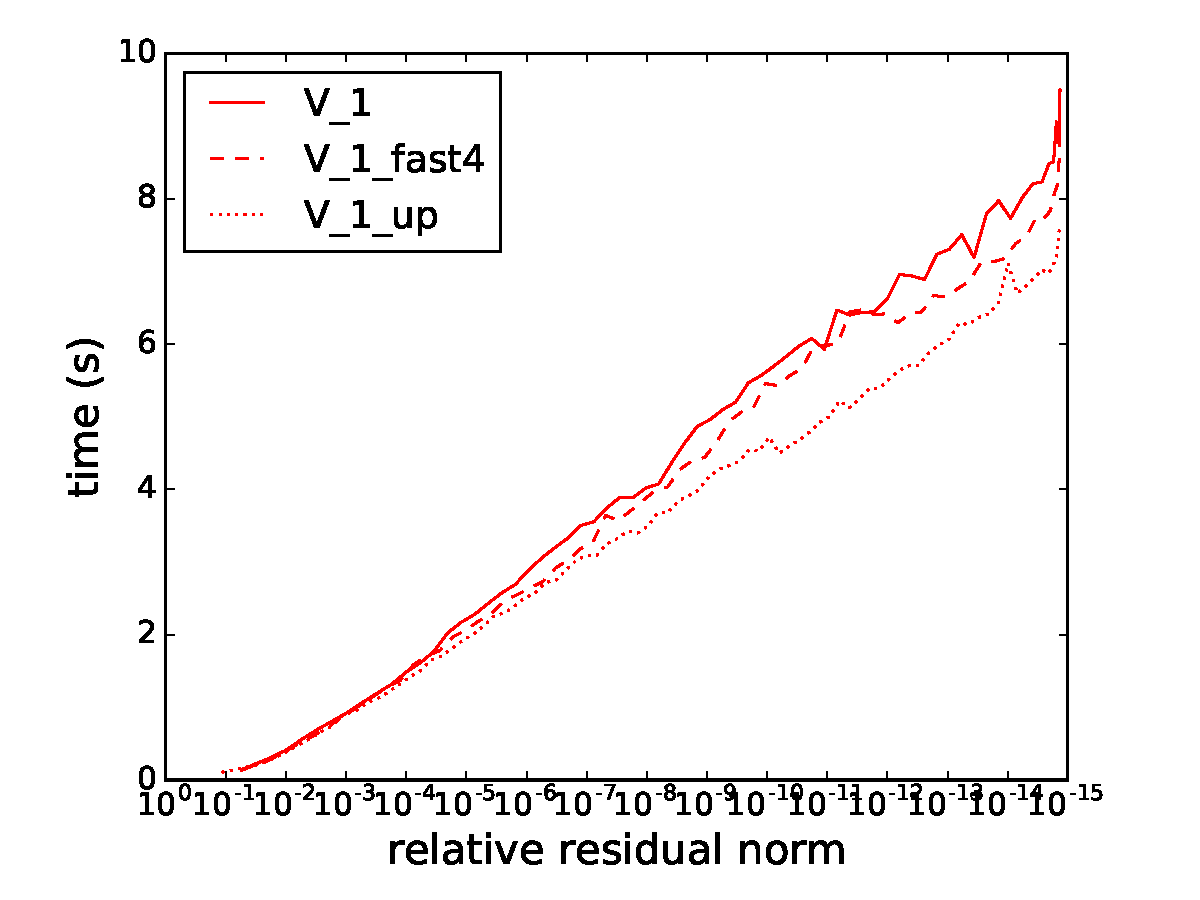
\includegraphics[width=0.45\linewidth]{figs/time_convergence_up_1.pdf}}
    \subfloat[\textsc{3DLaplace-9pt(1,1,1)}]{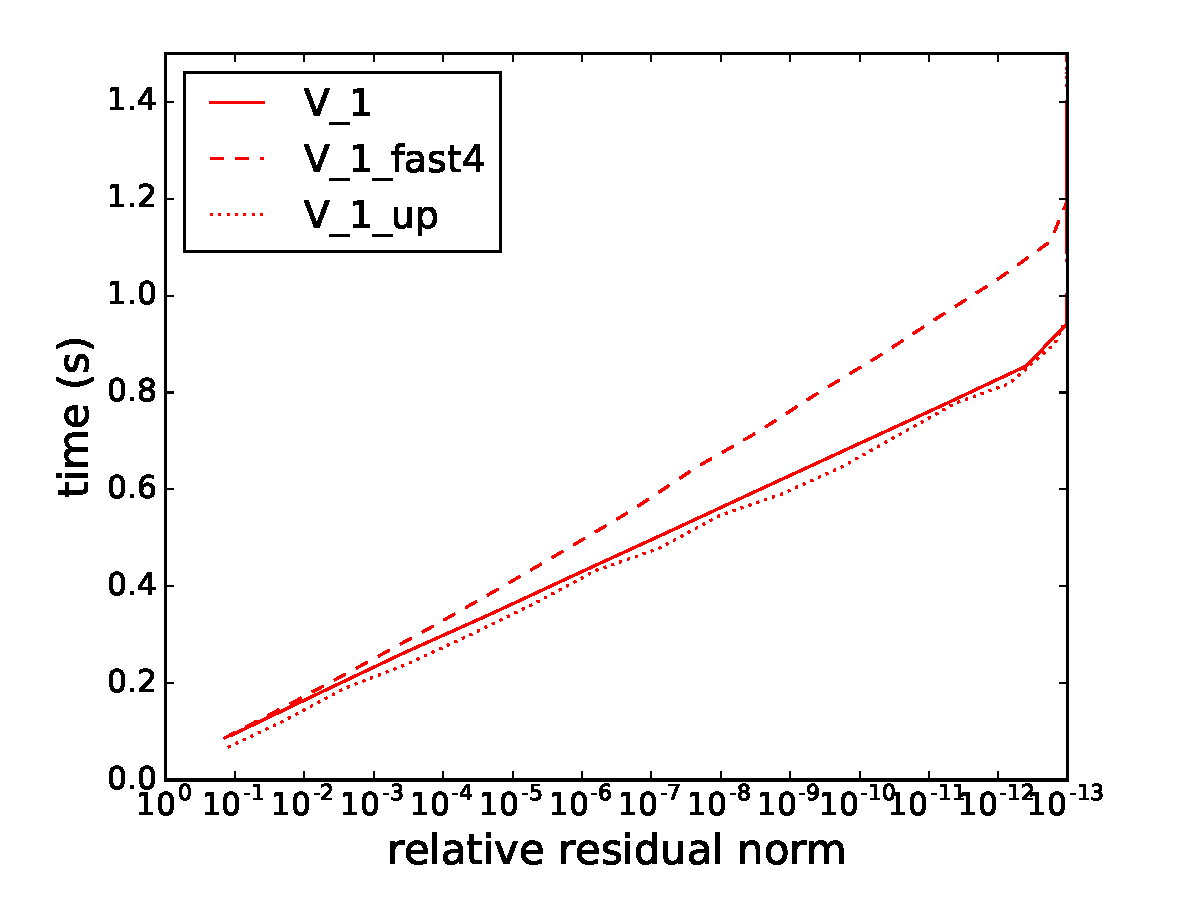
\includegraphics[width=0.45\linewidth]{figs/time_convergence_up_2.pdf}}\\
    \subfloat[\textsc{3DLaplace-9pt(0.1,0.1,0.01)}]{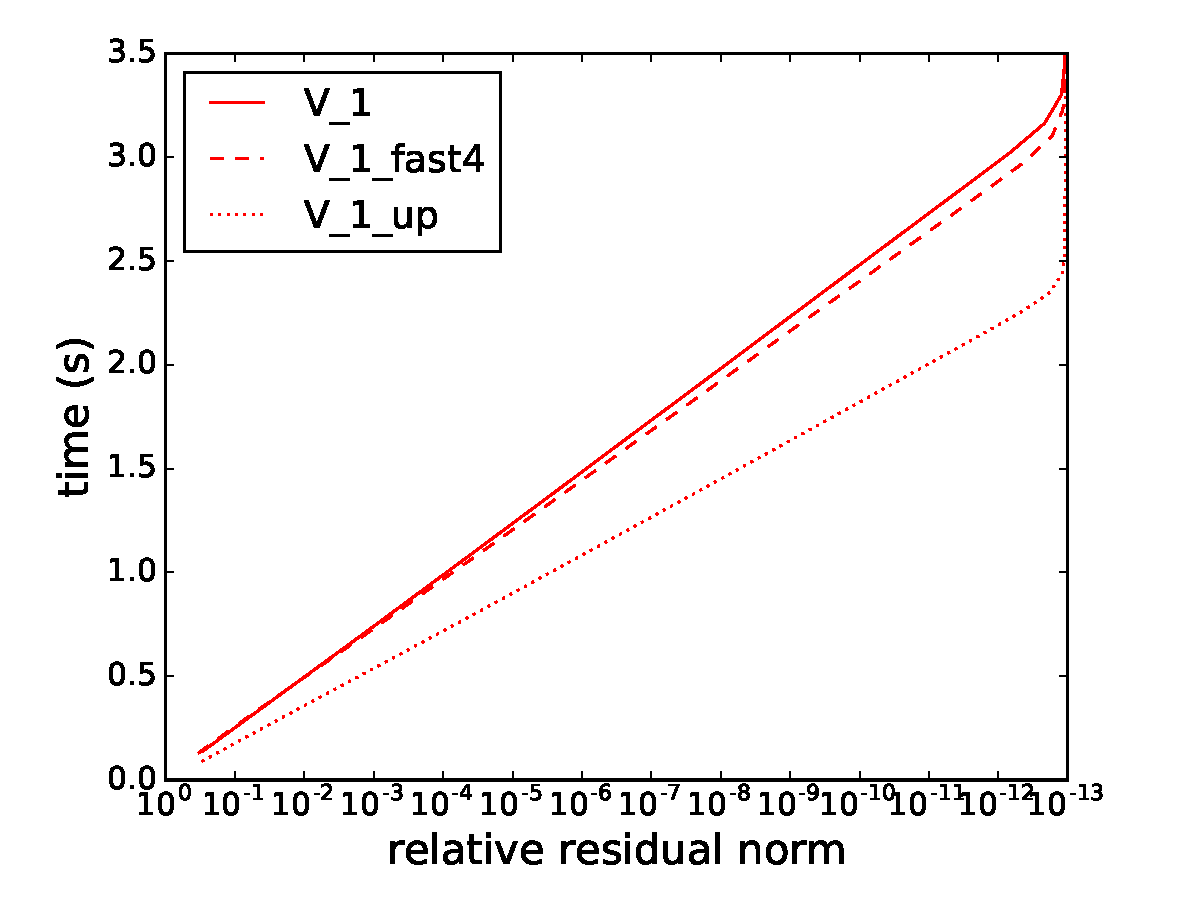
\includegraphics[width=0.45\linewidth]{figs/time_convergence_up_5.pdf}}
    \subfloat[\textsc{3DLaplace-9pt(5,5,5)}]{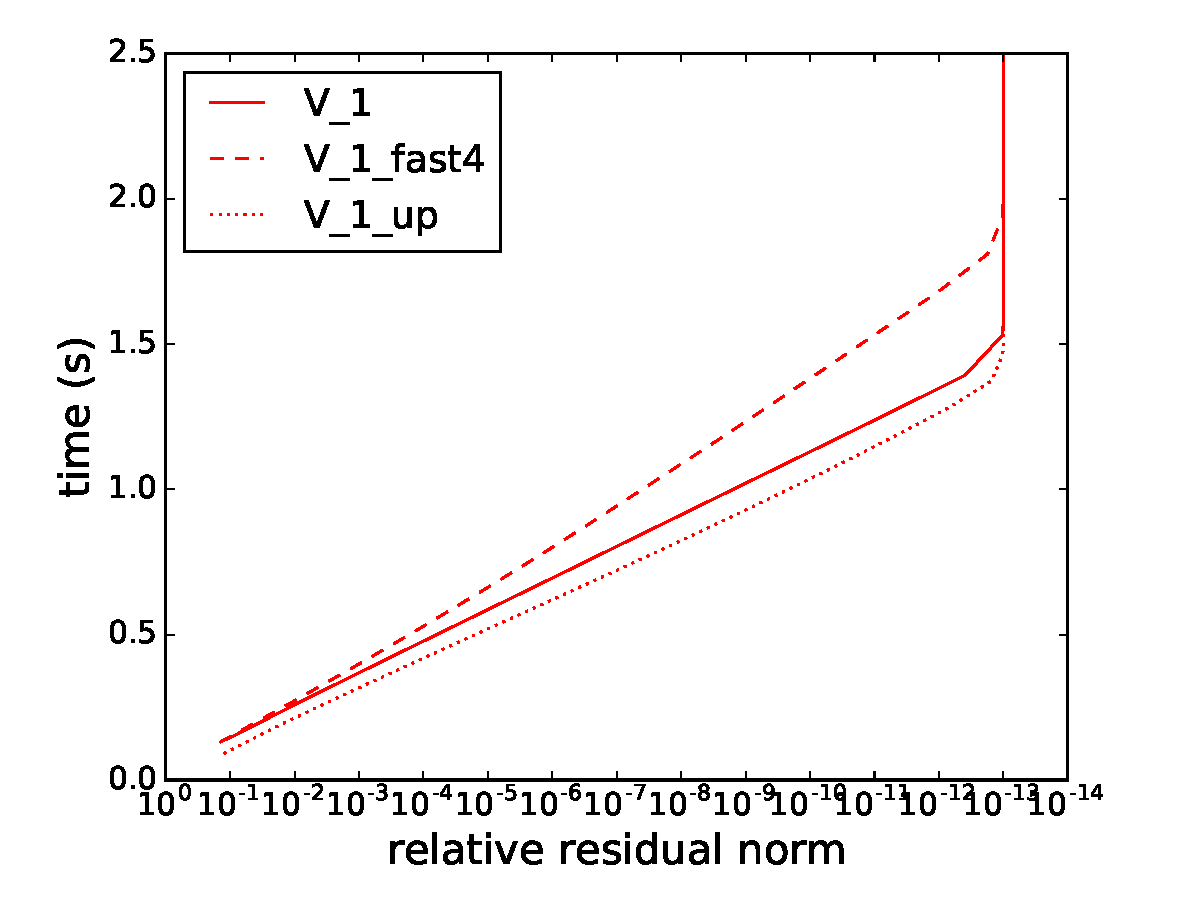
\includegraphics[width=0.45\linewidth]{figs/time_convergence_up_6.pdf}}\\
    \subfloat[\textsc{3DLaplace-27pt}]{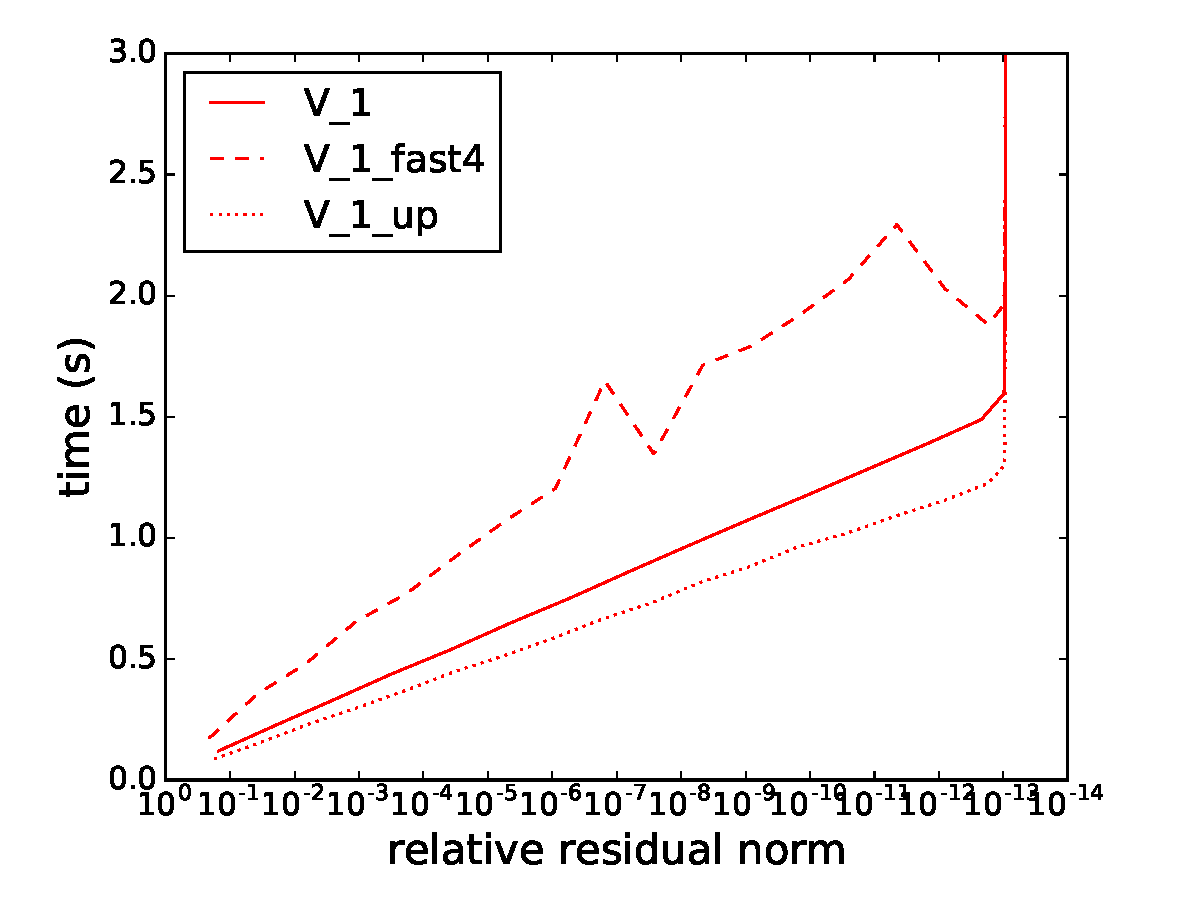
\includegraphics[width=0.45\linewidth]{figs/time_convergence_up_3.pdf}}
    \subfloat[\textsc{PDE-Dirichlet}]{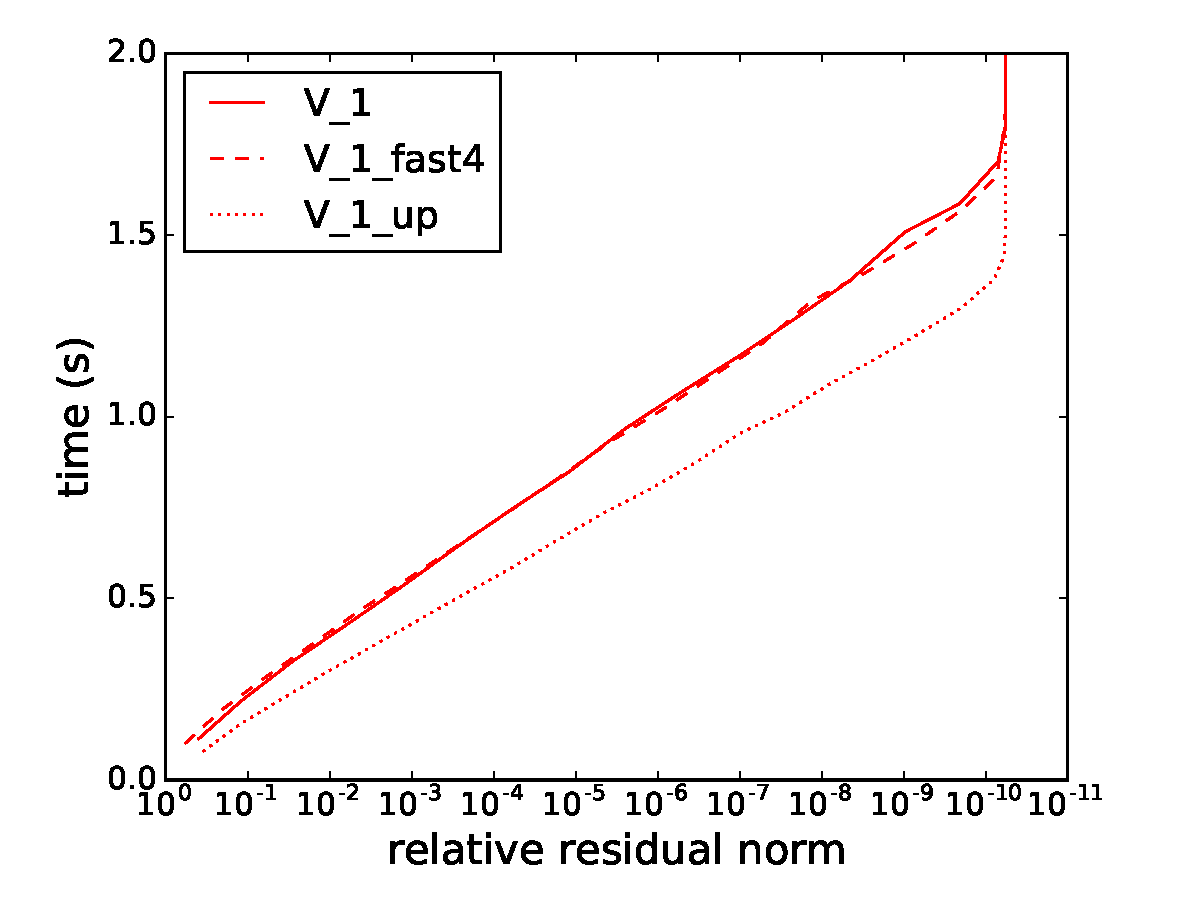
\includegraphics[width=0.45\linewidth]{figs/time_convergence_up_4.pdf}}
    \caption{Comparison of the original algorithm V1 with \emph{Fast4} and \emph{Up} strategies.}
    \label{fig.up_comparison}
\end{figure*}

The first thing we observe is that the \emph{Fast4} strategy does not
always perform well. In fact, for two of these four applications the
convergence rate is significantly slower than the classic V1 strategy.
However, the \emph{Up} strategy seems to be quite efficient; it improves
convergence speed by $12\%$,$7\%$,$20\%$ and $22\%$ for
\textsc{Unstructured-Anisotropy}, \textsc{3DLaplace-9pt},
\textsc{3DLaplace-27pt(1,1,1)} and \textsc{PDE-Dirichlet} respectively.

Given these positive results, we extended further our evaluation from
single-node runs to distributed executions in multiple nodes, in order to test
the viability of the \emph{Up} strategy when the algorithm is parallelized and
distributed. Larger cases were tested on a cluster with 100 compute nodes, 
each node equippred with 2 Intel Xeon E5-2630 v3 Haswell 8-core processors, 
each core at 2.4 GHz, and with 20 MB L3 cache.
%Each node is equipped with 2 Intel processors, 2 nvidia GPUs, over 20GB of DRAM
%and all connected through an Infiniband network.}

The total size of the matrix is set to either 5,832,000 or 13,824,000, while
the topology is composed of either 27 (3x3x3), 36 (6x6x1) or 64 (4x4x4)
processors, where each processor holds 1 MPI process and runs 1 OpenMP
thread per process. The problems tested are \textsc{3DLaplace-9pt} and
\textsc{3DLaplace-27pt}.  For these 6 possible combinations, we observe an
average improvement of 18.4\% (ranging from 16.0\% to 28.3\%) for
\textsc{3DLaplace-9pt} and 20.5\% (ranging from 16.2\% to 25.0\%) for
\textsc{3DLaplace-27pt}. It seems that \emph{Up} outperforms the
classical V-cycle even more when the problem size increases, but seems to cap at around
25\% improvement. Figure~\ref{fig.mtup} presents the results for the matrix
size 13,824,000 and \textsc{3DLaplace-27pt}, for the 3 different processor
topologies. Similar results are obtained for the other applications but are not
shown here for brevity.

\begin{figure*}[t]
    \subfloat[3x3x3]{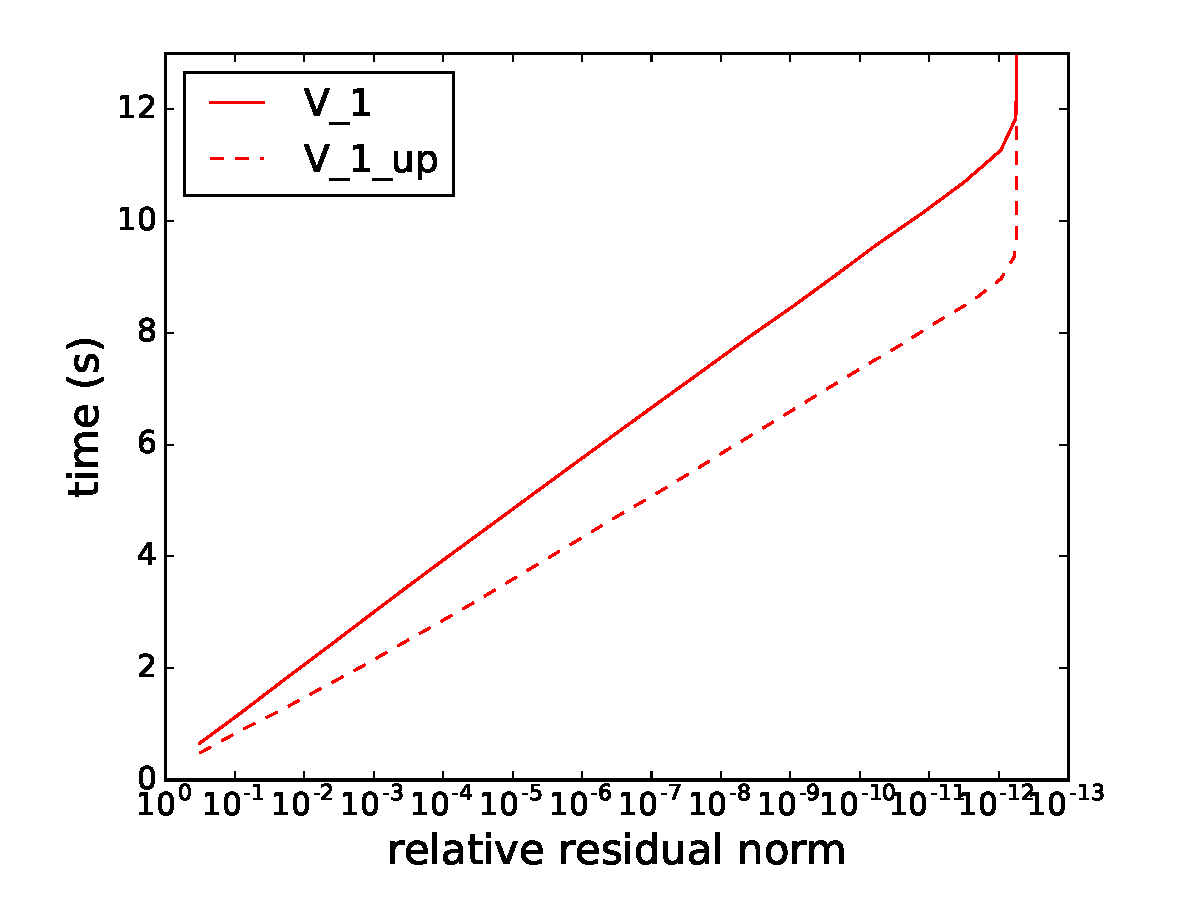
\includegraphics[width=0.33\linewidth]{figs/mt_27.pdf}}
    \subfloat[6x6x1]{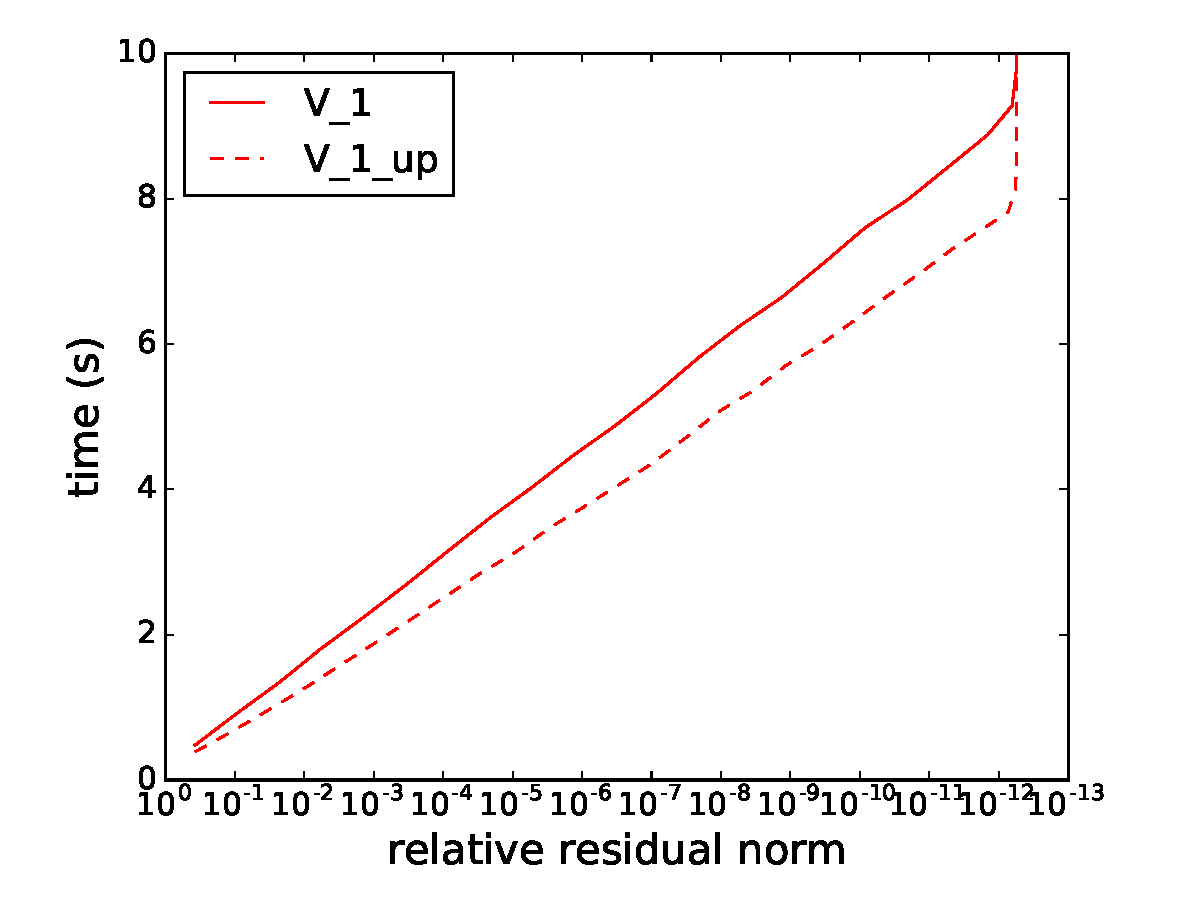
\includegraphics[width=0.33\linewidth]{figs/mt_36.pdf}}
    \subfloat[4x4x4]{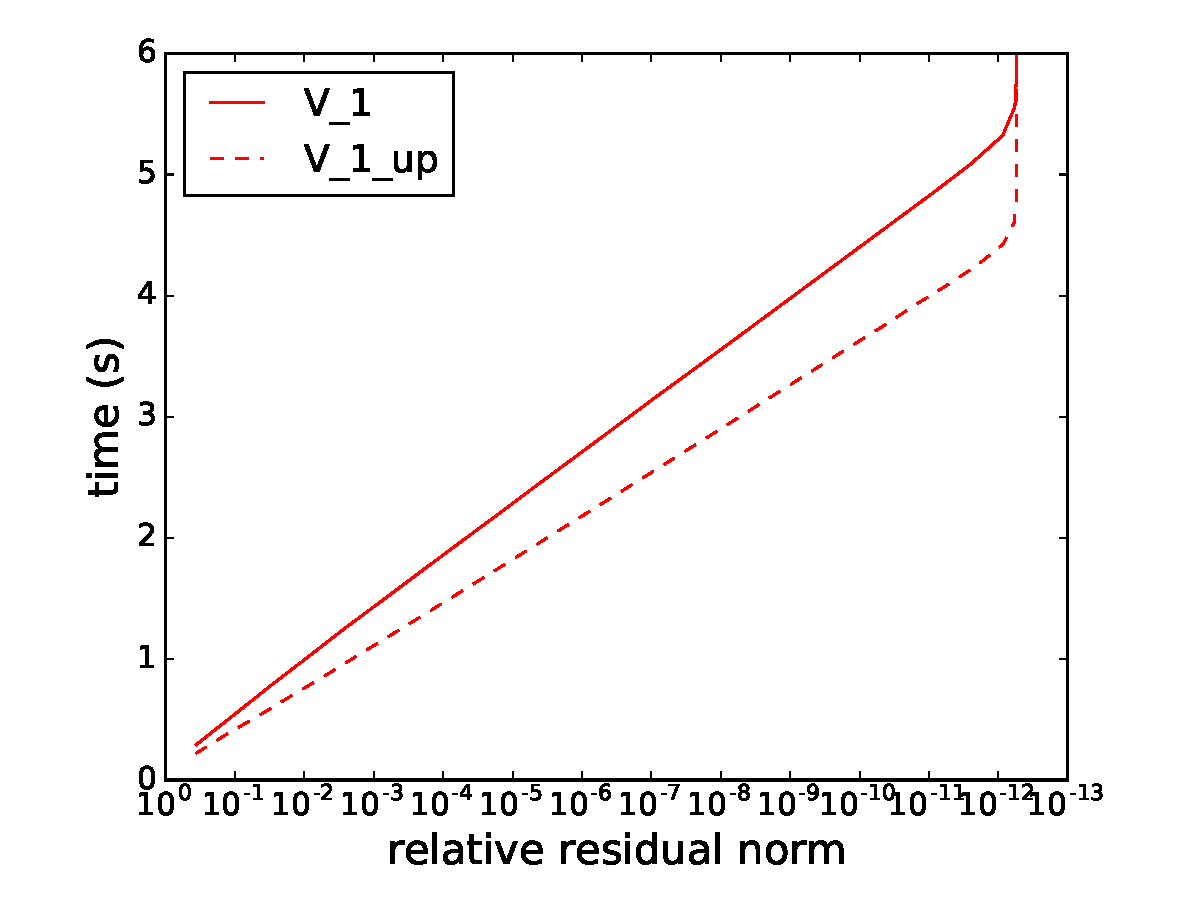
\includegraphics[width=0.33\linewidth]{figs/mt_64.pdf}}
    \caption{Comparison of original algorithm V1 with \emph{Up} strategy for
    \textsc{3DLaplace-27pt} on a 240x240x240 grid with different processor topologies.}
    \label{fig.mtup}
\end{figure*}


